\documentclass[12pt, a4paper]{article}
\usepackage[utf8]{inputenc}
\usepackage[italian]{babel}
\usepackage{fancyhdr} %Header e Footer
\usepackage{titling} %Spaziatura Titolo
\usepackage{enumitem}
\usepackage{setspace} 
\usepackage{siunitx} %Notazione scientifica e unità di misura
\usepackage{parskip} %Spaziatura paragrafi automatica
\usepackage{graphicx} %Imaggini
\usepackage{float} 
\usepackage{booktabs}
\usepackage[
    top=3cm,    
    bottom=2cm, 
    left=1.5cm,   
    right=1.5cm,
    headheight=15pt]{geometry} %Margini
\usepackage[colorlinks=true, linkcolor=cyan]{hyperref} %Colore link
\usepackage{amsmath}
\usepackage[italian, capitalize]{cleveref} %Nuovo nome refernce
\usepackage{caption}

\setstretch{0.85}
\title{2° Esperienza Laboratorio di Fisica 2} %NUMERO ESPERIENZA   
\author{Gruppo B02: Bifulco Flavio DC6000147 - De Marco Alessandro DC6000138 - \\ De Simone Adriano DC6000154}
\date{14/10/2026} %DATA
\setlength{\droptitle}{-2cm}

% Titolo in grassetto e riduzione spazio sotto 
\pretitle{\begin{center}\huge\bfseries} 
\posttitle{\par\end{center}} 

% Autore più piccolo 
\preauthor{\begin{center}\small} 
\postauthor{\par\end{center}}

\postdate{
    \par\end{center} 
    \vspace{0.5em}   
    \begin{center}
        \textit{\textbf{\Large Stima di una resistenza con metodo il Volt-Amperometrico}} %TITOLO
    \end{center}
    \vspace{0.5cm} 
}

\newcommand{\E}{\`E } % Comando per "è" grande

\graphicspath{{./immagini/}}
\renewcommand{\thefigure}{\arabic{section}.\arabic{figure}}
\addto\captionsitalian{\renewcommand{\figurename}{Immagine}}
\crefname{figure}{Immagine}{immagini}
\makeatletter
\@addtoreset{figure}{section}
\makeatother

\pagestyle{fancy}
\fancyhf{}

% Configurazione Header
\fancyhead[L]{Gruppo B02: Bifulco Flavio - De Marco Alessandro - De Simone Adriano}       
\fancyhead[R]{\thedate}                
\renewcommand{\headrulewidth}{0pt}
\addtolength{\headsep}{10pt}

% Configurazione Footer
\fancyfoot[C]{\thepage} 

\sisetup{
    output-decimal-marker = {,},
    separate-uncertainty = true,
    per-mode = fraction
}
\DeclareSIUnit\cal{cal}

\renewcommand{\thesection}{\arabic{section})}
\renewcommand{\thesubsection}{\arabic{section}.\arabic{subsection})}
\renewcommand{\thesubsubsection}{\arabic{subsubsection})}
\renewcommand{\theHsection}{\arabic{section}}
\renewcommand{\theHsubsection}{\arabic{section}.\arabic{subsection}}
\renewcommand{\theHsubsubsection}{\arabic{section}.\arabic{subsection}.\arabic{subsubsection}}
\hypersetup{bookmarksnumbered}
\begin{document}
\maketitle
%\textbf{\Large Obiettivo:}
%\begin{enumerate}[label=\arabic*), leftmargin=2cm]
%    \item Verifica sperimentalmente la prima legge di Ohm con il metodo volt-amperometrico. 
%\end{enumerate}
%
%\textbf{\Large Strumentazione:}
%\begin{itemize}[label= -, leftmargin=2cm]
%    \item Bilancia (\(\Delta G_\text{sens} = \qty{0.1}{\gram}\)).
%    \item 
%\end{itemize}
%
%\bigskip \bigskip
%\noindent{\LARGE \textbf{Procedimento di misura e analisi dati: }}\(\)
%\bigskip

\section{Introduzione}

\section{Apparato sperimentale}
\begin{itemize}[leftmargin=2cm]
    \item 
\end{itemize}


\section{Ponte di Wheatstone}
\subsection{Introduzione}
Per misurare una resistenza incognita del ponte di Wheatstone si è ricercata la condizione di 
bilanciamento del ponte. Per fare ciò è stato utilizzato un amperometro analogico per misurare il 
flusso di corrente tra i due lati del ponte e un resistore variabile per modificare la condizioni del
ponte. Una volta ottenute varie misure della corrente al variare della resistenza variabile, si 
effettua un fit per stimare in maniera più precisa la condizione di equilibrio, dove la resistenza 
variabile corrisponderà alla resistenza incognita.

Alla condizione di bilanciamento si verifica: \(R_4 = \frac{R_2 \cdot R_3}{R_1}\)

\subsection{\textbf{Misure acquisite}}

\E stato realizzato un circuito elettrico utilizzando la basetta e icavi a disposizione. Il resistore 
\(R_0 = \qty{4.69(0.01)}{\kilo\ohm}\) di protezione è stato inserito per limitare la corrente nel 
circuto.

\begin{figure}[H]
    \centering
    \caption{Ponte di Wheatstone}
    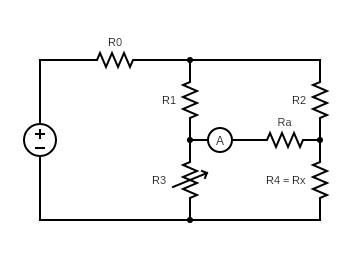
\includegraphics[width=0.5\textwidth]{ponte_wheatstone.png}
    \label{fig:ponte_wheatstone}
\end{figure}

Il generatore di tensione è stato impostato per erogare una d.d.p. costante pari a 
\(V_0 = \qty{15}{\volt}\), il fondoscala dell'amperometro è stato impostato su \qty{500}{\micro\ampere}.
Dopo aver effettuato una scansione rapida della resistenza variabile, per trovare una regione approssimata 
della condizione di bilanciamento del ponte, si è proceduto variando la resistenza con un passo di \qty{10}{\ohm}
tra un valore minimo di \qty{240}{\ohm} e un valore massimo di \qty{310}{\ohm}. L'incertezza delle 
misure della resistenza variabile è stata presa come l'1\% (come indicato sul resistore variabile), 
mentre per le misure della corrente è stata usata la formula \(\sigma = \frac{\delta}{\sqrt{12}}\) per
trasformare gli errori massimi in errori statistici.

I valori delle resistenze \(R_1 = \qty{220(0.6)}{\ohm}\) e \(R_2 = \qty{118.9(0.4)}{\ohm}\) sono stati
misurati utilizzando l'RCL meter e le loro incertezze caclolate utilizzando la formula data dal costruttore.

Di seguito sono riportati i valori misurati:

\begin{table}[H]
\centering
\begin{tabular}{@{}llll@{}}
\toprule
R(\(\Omega\)) & I(\(\unit{\micro\ampere}\)) & \(\Delta\)R(\(\Omega\)) & \(\Delta\)I(\(\unit{\micro\ampere}\)) \\ \midrule
240         & 8.0   & 2                   & 0.3           \\
250         & 6.0   & 3                   & 0.3           \\
260         & 4.0   & 3                   & 0.3           \\
270         & 1.5   & 3                   & 0.3           \\
280         & -1.5  & 3                   & 0.3           \\
290         & -3.5  & 3                   & 0.3           \\
300         & -6.0  & 3                   & 0.3           \\
310         & -8.0  & 3                   & 0.3           \\ \bottomrule
\end{tabular}
\end{table}

\subsection{\textbf{Analisi dati}}


%\renewcommand{\thesection}{}
%\renewcommand{\thesubsection}{\arabic{subsection})}
\section{Conclusioni} %Conclusioni

\end{document}
